\documentclass[a4paper]{article}
\usepackage{dirtytalk}
\usepackage{graphicx}
\usepackage[hidelinks]{hyperref}
\usepackage{xcolor}
\usepackage{url}
\usepackage{animate}
\usepackage{outlines}
\usepackage{listings}
\usepackage{fontspec}
\lstset{basicstyle=\ttfamily,
	showstringspaces=false,
	commentstyle=\color{blue},
	keywordstyle=\color{pink}
}
\lstset{emph={
	EXPOSE,RUN,FROM,CMD,nc,tcp,udp,http,docker},emphstyle=\color{purple}
}
\newcommand{\abc}{\hfill \break}
\usepackage{fancyhdr}
\usepackage{geometry}
\geometry{
	a4paper,
	total={170mm,257mm},
	left=20mm,
	top=20mm,
	bottom=39mm,
}

\setlength{\headheight}{82.70538pt}

\fancypagestyle{oida}{
	\fancyhf{}
	\fancyhead[L]{\fontsize{7.5}{7.5}htl donaustadt\\ Donaustadtstraße 45\\
		1220 Wien\\~\\ Abteilung: Informationstechnologie\\ 
	Schwerpunkt: Netzwerktechnik}
	\fancyhead[R]{
\includegraphics[scale=0.45]{images/logo.png}}

	\fancyfoot[L]{\today}
	\fancyfoot[C]{\jobname}
	\fancyfoot[R]{Page: \thepage}
}

\begin{document}
\bibliographystyle{IEEEtran}
\pagestyle{oida}
\section*{Capturing of network traffic in the local
network}
\par\noindent\rule{\textwidth}{0.4pt}

Laboratory protocol
Excercise 10: Capturing of network traffic in the local
network

\begin{figure}[h]
	
\includegraphics[scale=0.5]{images/mencicle.png}
	\caption{Grouplogo}
	\centering
\end{figure}

\vspace*{\fill}
Subject:	ITSI

Class:	3AHITN

Name:	Stefan Fürst, Justin Tremurici

Gruppenname/Nummer: Name here/12

Supervisor: 	SPAC, ZIVK

Exercise dates:	11.04.2025 | 25.04.2025 | 09.05.2025

Submission date: 16.05.2025


\newpage
\tableofcontents

\newpage

\section{Task definition}

This task focused on the passive interception of network traffic in a local network using either a hub or a managed switch with mirror ports. The objective was to analyze unaltered communications using \texttt{Wireshark} on both attacker and victim machines. Two topologies were tested: a hub-based setup, which allowed full traffic visibility, and a switch-based setup, where traffic was mirrored from victim ports to the attacker’s port. Devices were assigned static IP addresses from a private range, and \texttt{VoIP} communication was simulated using either software-based or physical \texttt{IP} phones.\abc
Three types of traffic were examined: \texttt{ICMP} echo requests (Ping), \texttt{HTTP} authentication involving plaintext credentials, and \texttt{VoIP} calls between two endpoints. Each case was recorded in a separate \texttt{Wireshark} capture. In the hub scenario, the focus was on visibility and potential stability issues under high traffic. For the switch, mirroring was configured and traffic was captured before and after to assess changes.\abc
Further tasks involved filtering \texttt{ICMP} traffic by attacker \texttt{IP}, observing ping communication between victim devices from the attacker’s perspective, capturing \texttt{HTTP} login attempts to extract credentials, and intercepting a \texttt{VoIP} call, which was exported as an \texttt{MP3} file. All relevant captures and the audio file were submitted as part of the final documentation.\footnote{The task definition was created by ChatGPT.}

\section{Summary}
In this exercise, two distinct network topologies were implemented to investigate passive network traffic interception. The first topology utilized personal hardware, specifically a \texttt{Mikrotik RB5009} router, to configure port mirroring. The client devices were older laptops running \texttt{Proxmox}, with one laptop hosting an \texttt{nginx} container configured to demonstrate basic \texttt{HTTP} authentication. The attacker device was another laptop connected to the mirrored ports on the router, which allowed it to receive a complete copy of the network traffic between the clients and the server.\abc
The initial step involved performing local \texttt{ICMP} ping requests from the attacker to the clients to observe the captured traffic and verify network connectivity. Following this, the two client laptops pinged each other, while the attacker monitored and recorded the exchanged packets. This demonstrated the attacker's ability to intercept traffic not directly addressed to it due to the port mirroring setup. Furthermore, the attacker was able to capture and analyze the \texttt{HTTP} basic authentication process, successfully extracting plaintext credentials transmitted from the client to the \texttt{nginx} server.\abc
In the second part of the exercise, a \texttt{VoIP} call was established using two \texttt{IP} phones connected via a network hub instead of a switch with port mirroring. This topology allowed the attacker laptop to capture the audio stream of the call directly from the network traffic. The recorded audio was then exported and post-processed using \texttt{Audacity} and \texttt{Adobe Podcast Speech Enhancer} to clean and enhance the recording, resulting in a clear and intelligible audio file.\abc
Throughout the exercise, \texttt{Wireshark} was extensively used to capture, filter, and analyze the network traffic from the attacker’s perspective. This practical approach provided insight into how network devices like hubs and switches with port mirroring impact the visibility of traffic and the feasibility of passive interception attacks within a local network environment.\footnote{The summary was created after providing a draft of bullet points to ChatGPT.}

\newpage

\section{Complete network topology of the exercise}

\begin{figure}[ht]
	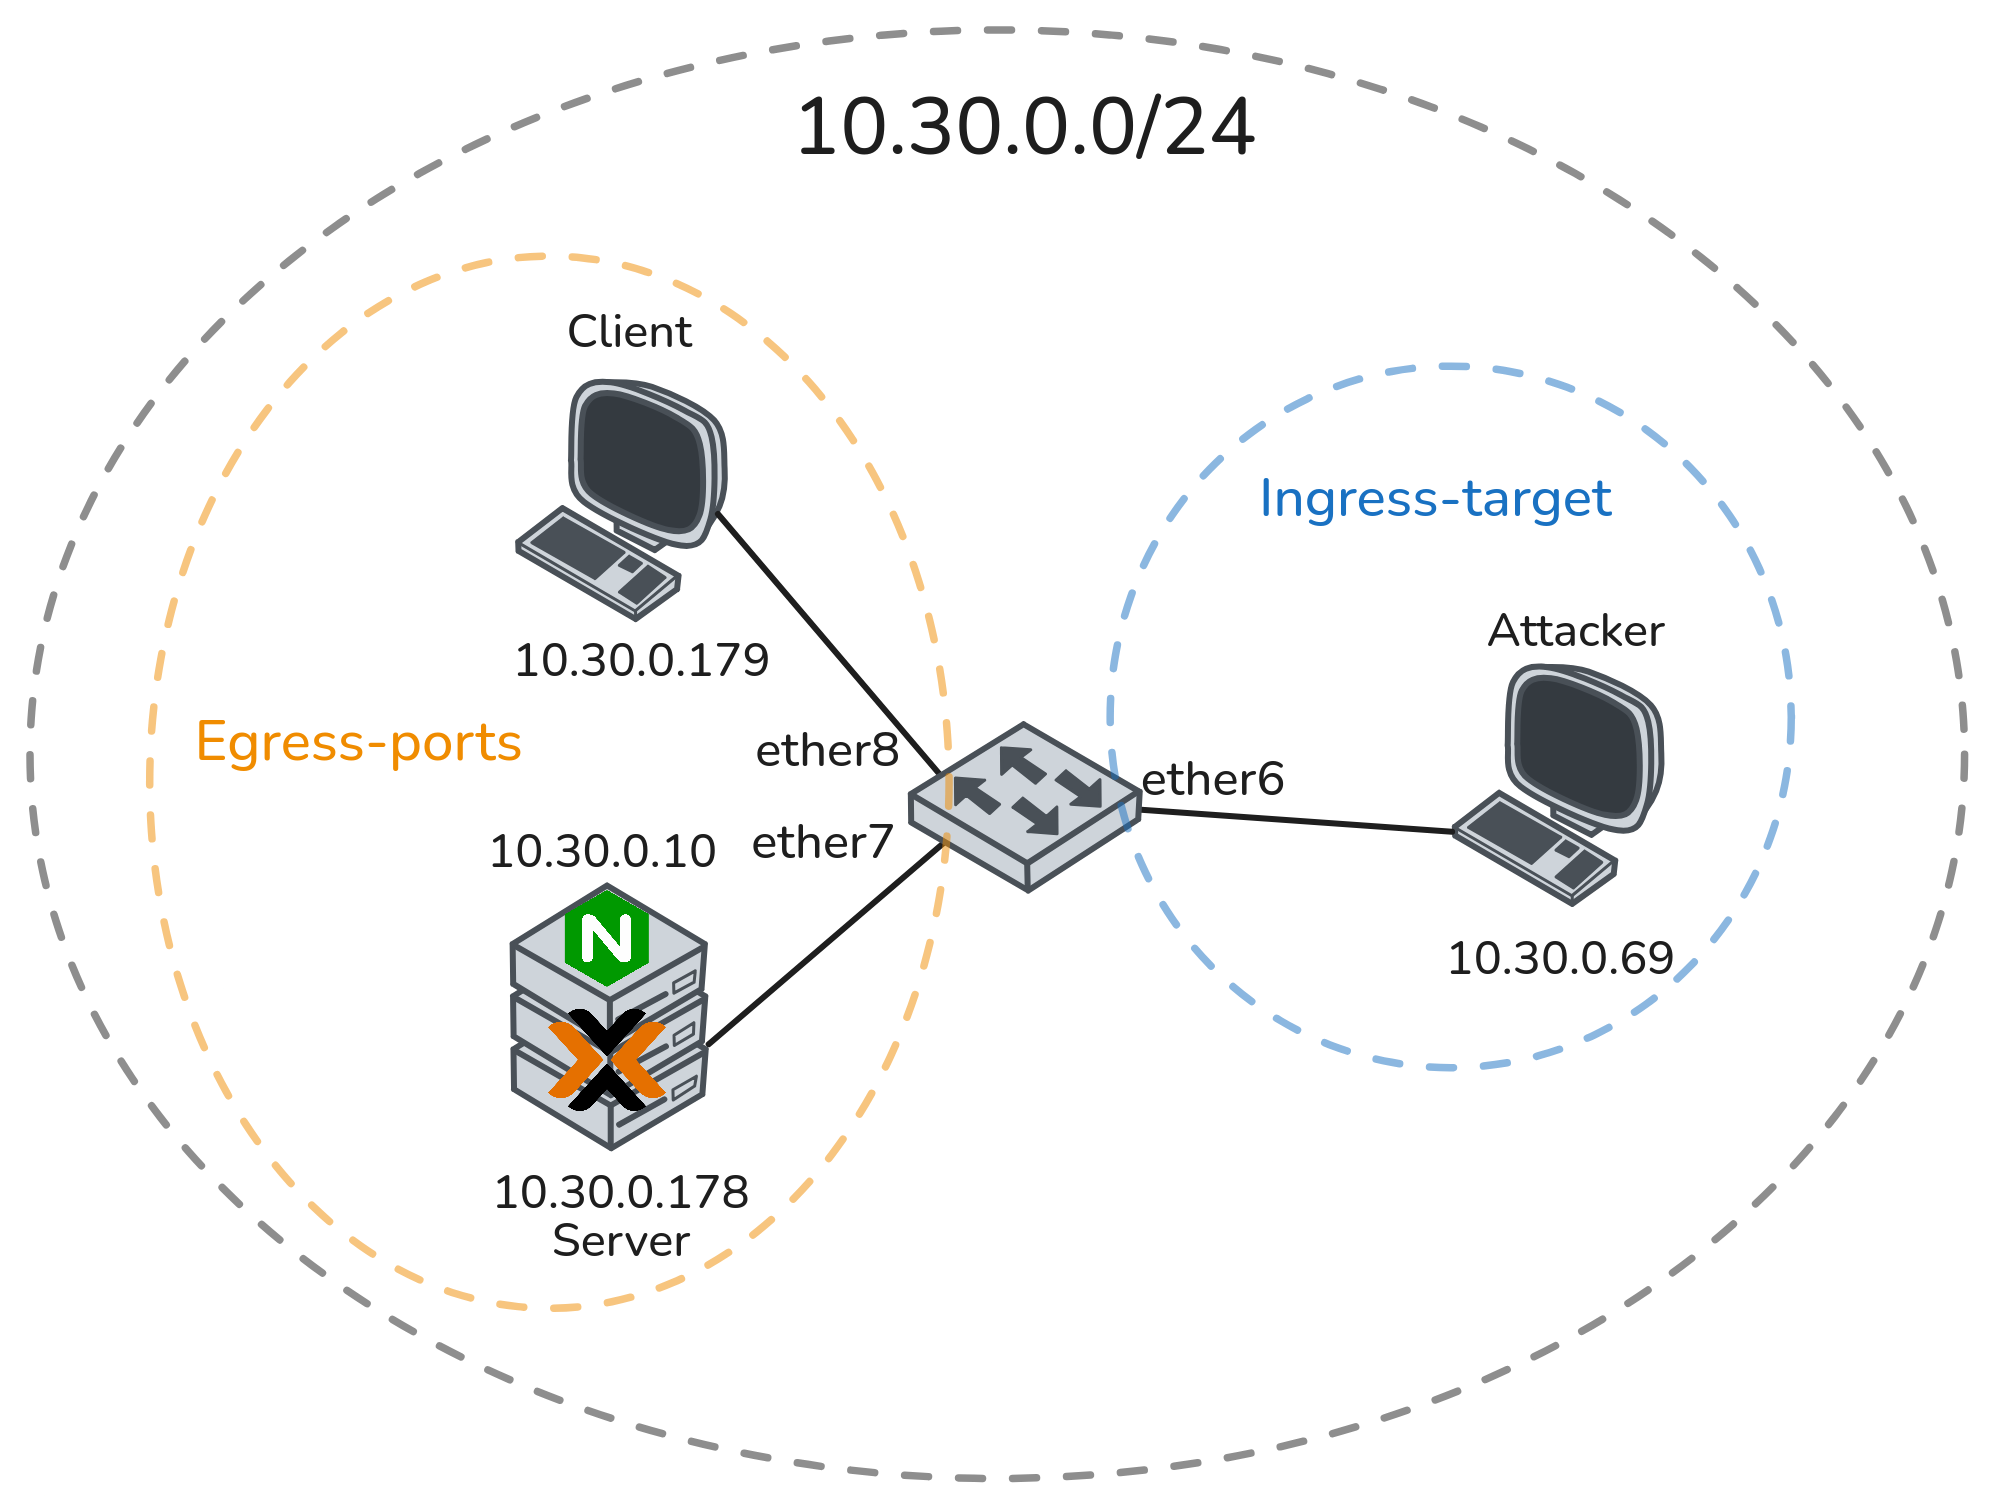
\includegraphics[scale=0.18]{images/topo1.png}
	\centering
	\caption{Complete network topology of the exercise using a switch}
	\label{fig:topo1}
\end{figure}
\begin{figure}[!htbp]
	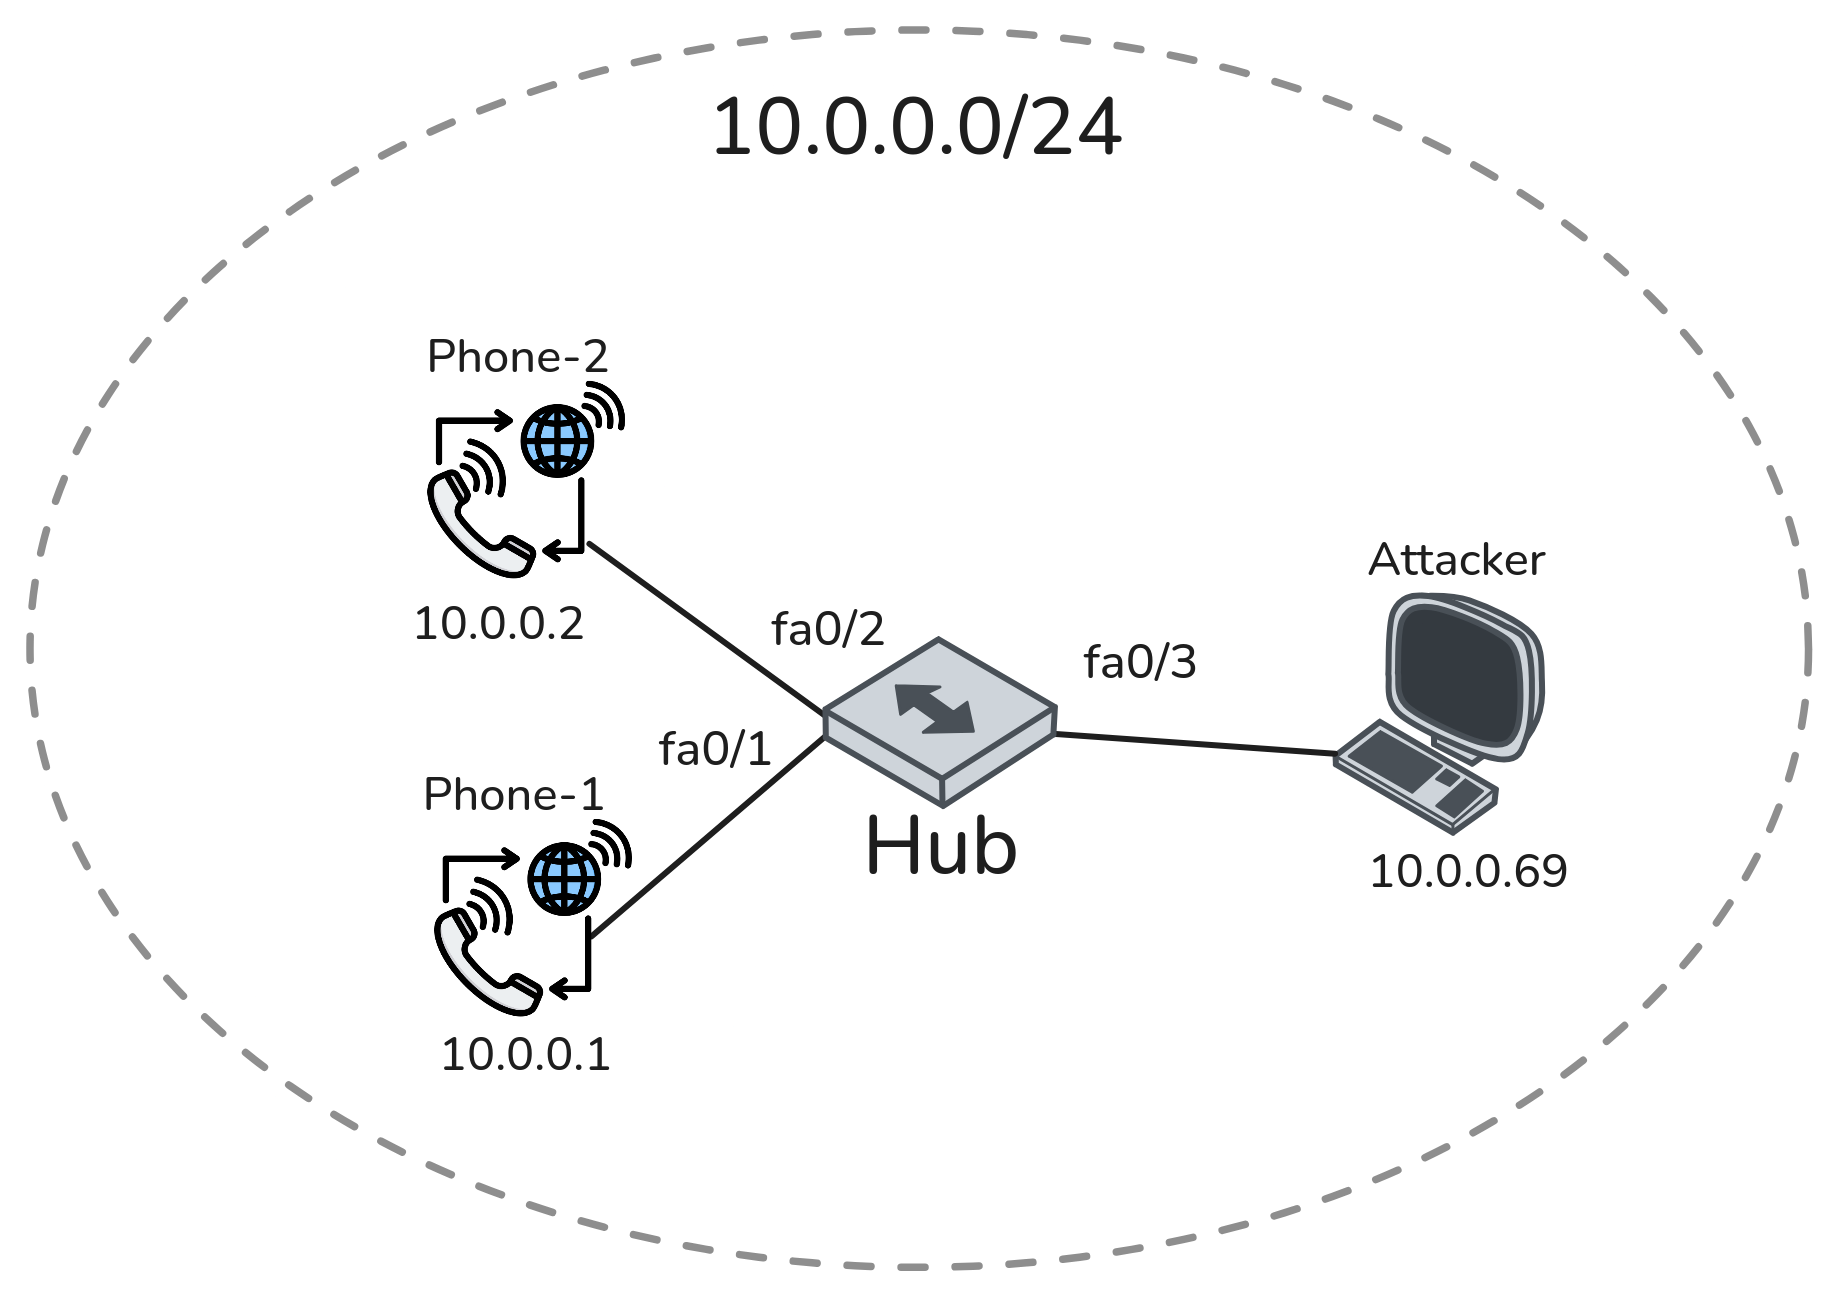
\includegraphics[scale=0.18]{images/topo2.png}
	\centering
	\caption{Complete network topology of the exercise using a Hub}
	\label{fig:topo2}
\end{figure}

\newpage

\section{Exercise Execution}

\subsection{Building the Topologies}

To build the topology from \textcolor{blue}{\hyperref[fig:nwconf]{Figure \ref{fig:topo1}}}, I chose the following hardware: a \texttt{Mikrotik RB 5009} to act as the main "switch" due to \texttt{RouterOS} offering extensive settings in what I consider the best GUI to manage any network device.\abc
% Additionally, I used an \texttt{Allied Telesis AT-FS980M/52FS POE} solely to power the router, since I didn't have more power plugs available.\abc
For the server and clients, I used two old laptops running Proxmox, one of which has a Debian server VM running an Nginx web server with basic authentication set up. All of the devices have static IPs configured in the range \texttt{10.30.0.0/24}. The attacker simply runs Linux with Wireshark to capture the traffic. The used IP addresses can be found in the addressing table below.

\begin{table}[h]
\centering
\begin{tabular}{|l|l}
\hline
\textbf{Deivce}    & \multicolumn{1}{l|}{\textbf{IP}}          \\ \hline
Attacker  & \multicolumn{1}{l|}{10.30.0.69}  \\ \hline
Server    & \multicolumn{1}{l|}{10.30.0.179} \\ \hline
Webserver & \multicolumn{1}{l|}{10.30.0.10}  \\ \hline
Client    & \multicolumn{1}{l|}{10.30.0.179} \\ \hline
\end{tabular}
\caption{Addressing Table}
\label{tab:addressing-table}
\end{table}

\subsubsection{Mirroring traffic in \texttt{RouterOS v7}}
To configure the router, there are three options: either use the WebGUI, SSH into it, or use their program called \texttt{WinBox}, which is the option I went with. After connecting a port on the router, it automatically detects available ports, and I can simply select one of them and configure everything as needed via the MAC address, as seen in Figure 4.\abc
Note that it shows \texttt{192.168.88.1}, which is the default \texttt{IP} of the router, but this won't be used, as all the devices already have their network setup. It can therefore be ignored, since no additional configuration with VLANs is needed—it's just plug and play.

\begin{figure}[!htbp]
	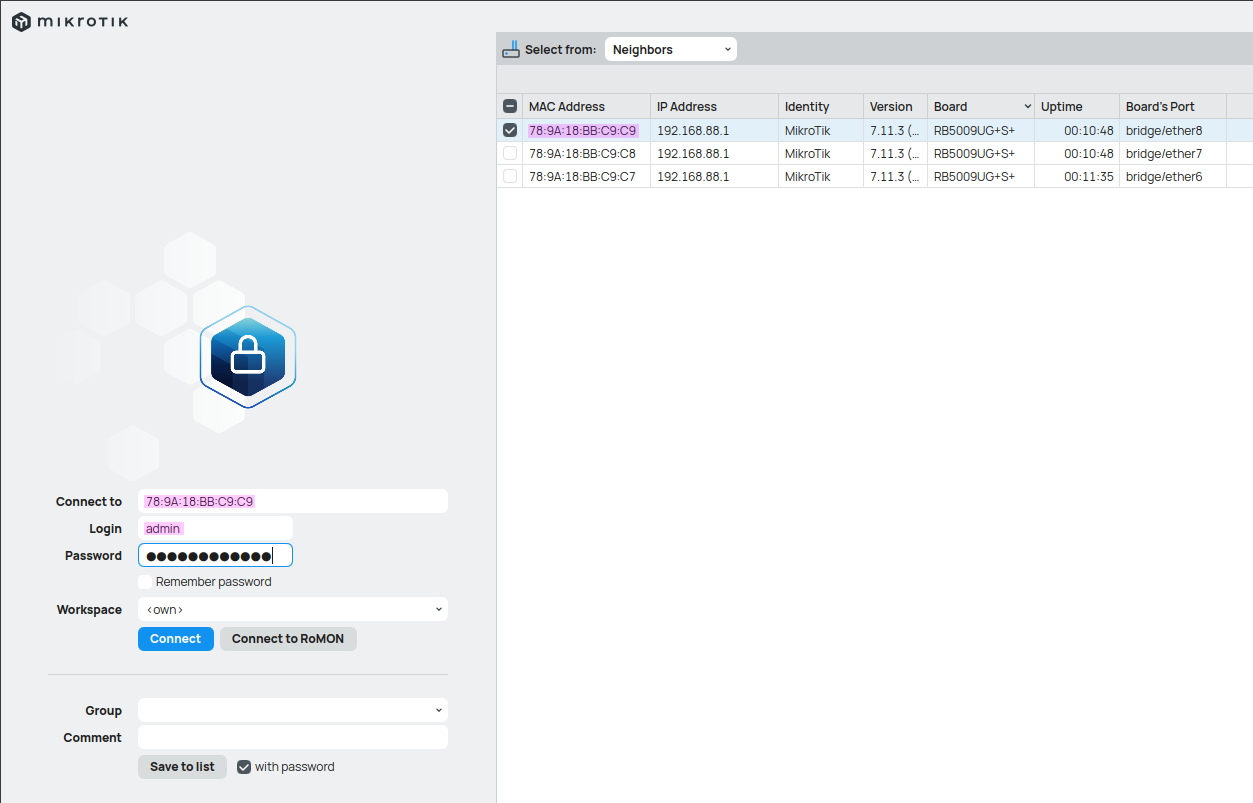
\includegraphics[scale=0.31]{images/winbox.png}
	\centering
	\caption{Connecting to the Router via \texttt{Winbox}}
\end{figure} \abc\newpage\abc
Now that we are in the router's configuration, we see a number of top-level options to choose from. To mirror traffic, we go to the \texttt{Switch} section and head to the \texttt{Port} tab, where we select the ports we want to mirror. If we double-click on an interface, it opens the port window, where we can choose whether to mirror only ingress traffic, egress traffic, or both.\abc
We also specify an ingress target, which in this case is \texttt{ether6}, where the attacker's laptop is plugged in so that it receives all the mirrored traffic. The configuration for both \texttt{ether7} and \texttt{ether8} is the same, which is why only one is shown in Figure 5 below. Lastly, under the "Mirror Ingress"/"Mirror Egress" columns in the switch window table, we can see a \texttt{yes} in both columns, indicating that the configuration has been successfully applied. \cite{mircotik-mirror}
\begin{figure}[!htbp]
	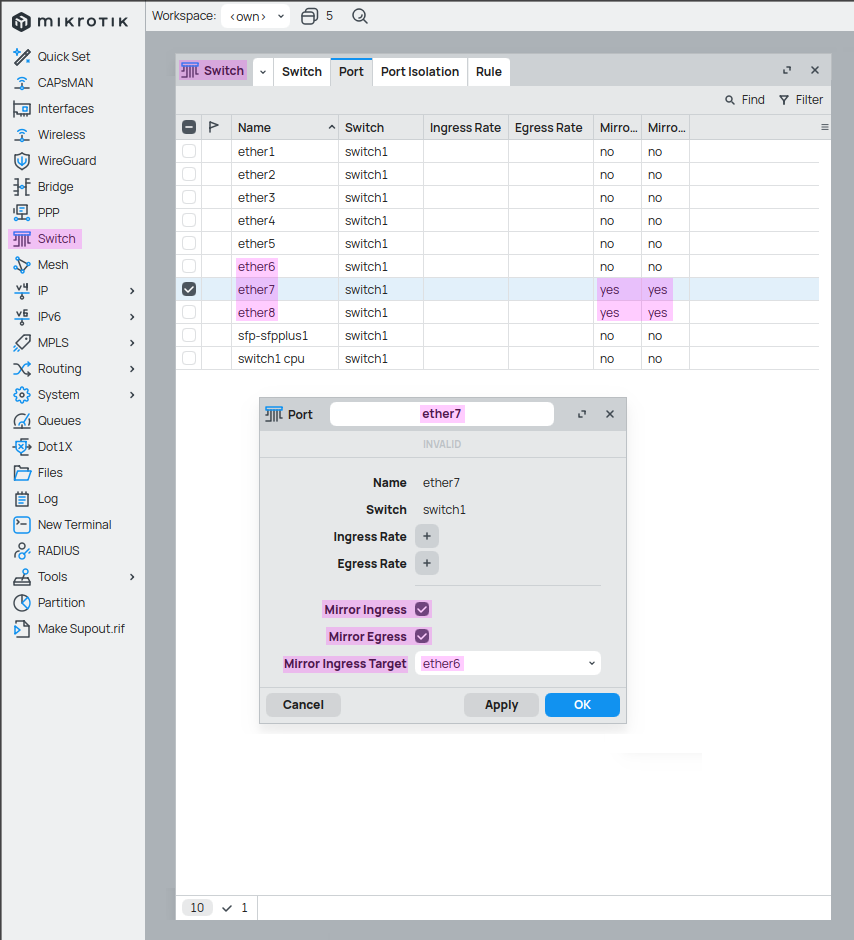
\includegraphics[scale=0.45]{images/routerconf.png}
	\centering
	\caption{Examining the traffic mirror configuration}
\end{figure} \abc\newpage
\subsubsection{Comparing the traffic before and after the configuarion}
Now we can use Wireshark on the attacker's laptop to compare the traffic captured with and without mirroring.\abc
When everything is idle and only \texttt{ARP} traffic is occurring in the background, the only difference is that instead of receiving each broadcast once, it is received twice—once from the connection itself and once from the mirroring.\abc
Figure 6 shows \texttt{ARP} traffic without mirroring, while Figure 7 shows it with mirroring, in which all the broadcasts appear twice. These duplicated frames either appear directly one after the other or with a few in between. The interruptions in frame order are caused by me having \texttt{WinBox} open, which continuously streams frames and therefore causes some variation in the captured frame sequence.
\begin{figure}[!htbp]
	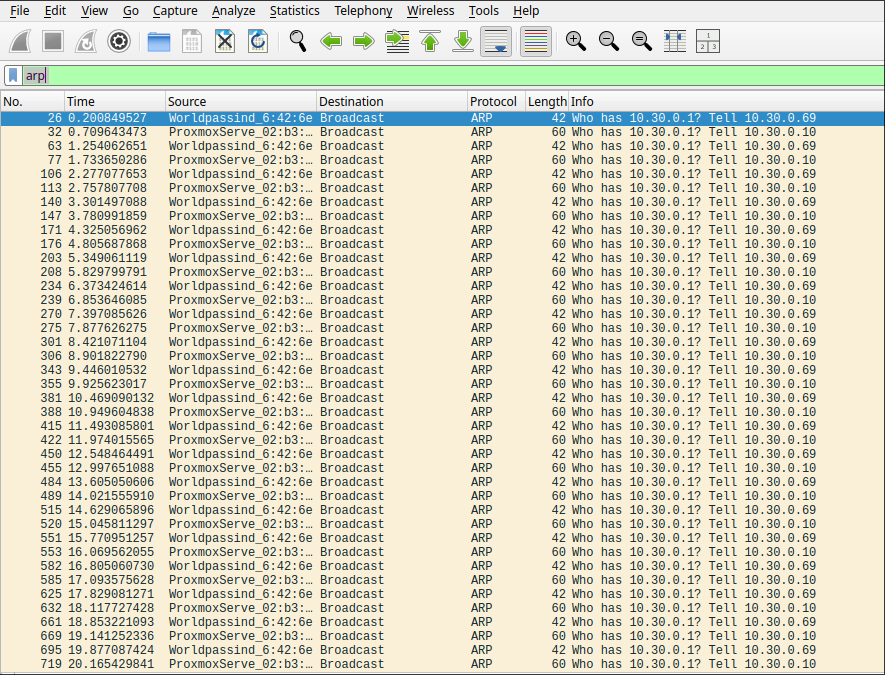
\includegraphics[scale=0.335]{images/nomirr.png}
	\centering
	\caption{Examining the \texttt{arp} traffic without a mirror configuration}
\end{figure} \abc
\begin{figure}[!htbp]
	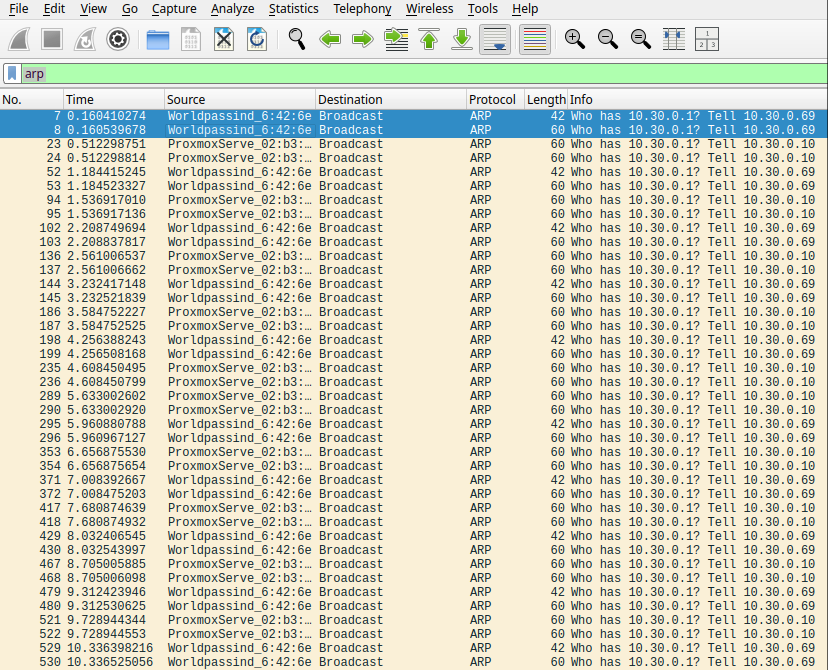
\includegraphics[scale=0.35]{images/yesmirr.png}
	\centering
	\caption{Examining the \texttt{arp} traffic with a mirror configuration}
\end{figure} \abc



\subsection{Packet Sniffing on the Local Device}
Now, with mirroring enabled, every device on the network is pinged so we can examine the behavior using the following filter: \texttt{ip.src == 10.30.0.69 \&\& icmp}. This filter shows only \texttt{ICMP} frames with the source IP of the attacker's laptop.\abc
The output of the filter displays all the issued ping requests, which can be verified in Figure 8 below.
\begin{figure}[!htbp]
	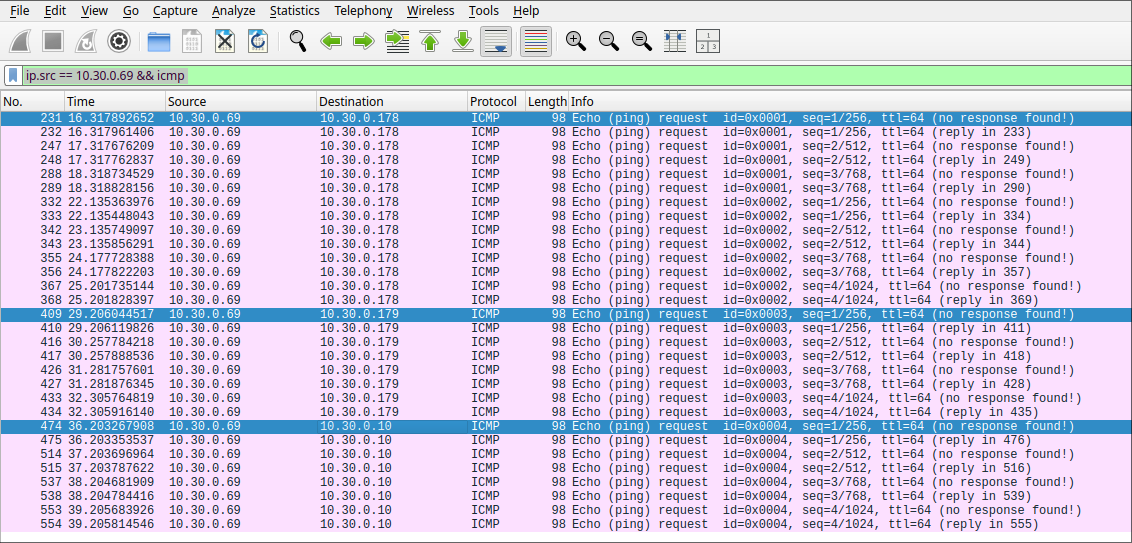
\includegraphics[scale=0.35]{images/ws2_1.png}
	\centering
	\caption{Displaying the pings to every device on the Network}
\end{figure} \abc
To display only the full connection between the two devices, the following filter can be used to show only the complete exchange, including replies: \texttt{icmp \&\& ip.addr == 10.30.0.69 \&\& ip.addr == 10.30.0.178}.\abc
This filter first includes only all \texttt{ICMP} frames, and then narrows it down to frames that involve both the IP address of the attacker's laptop and the target being pinged. This way, only the connection between the two—both requests and replies—is shown, as illustrated in Figure 9.

\begin{figure}[!htbp]
	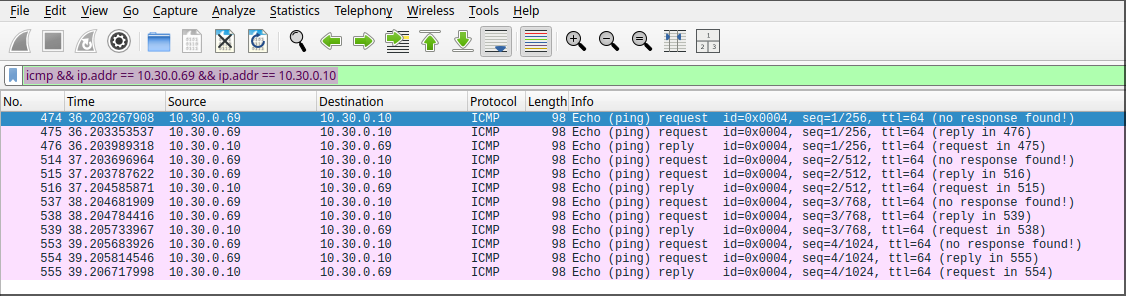
\includegraphics[scale=0.353]{images/filter for cumm.png}
	\centering
	\caption{Displaying the full ping between the attacker and a client}
\end{figure} \abc \newpage
\subsection{Capturing a Ping Between Two Targets}
Since all ingress and egress traffic is being mirrored to the attacker's port, it is possible to observe the entire ICMP exchange between the two victim machines directly from the attacker's PC using Wireshark. If a ping is initiated between the two devices, we can apply the same filter as before—replacing the IP addresses with those of the communicating victims—to capture and analyze the exchanged packets.\abc
\begin{quote}
\texttt{ip.addr == <Victim1\_IP> \&\& ip.addr == <Victim2\_IP>}
\end{quote}\abc
As shown in Figure 10, this traffic is visible \textbf{only} from the attacker's Wireshark capture. The source and destination fields in the packets correspond to the two victim machines—at no point does the attacker’s IP address appear in the captured communication. This interception is possible solely due to port mirroring: all network traffic to and from the mirrored ports is duplicated to the attacker's port. The two clients are unaware of this and communicate normally, while the attacker silently captures their traffic.
\begin{figure}[!htbp]
	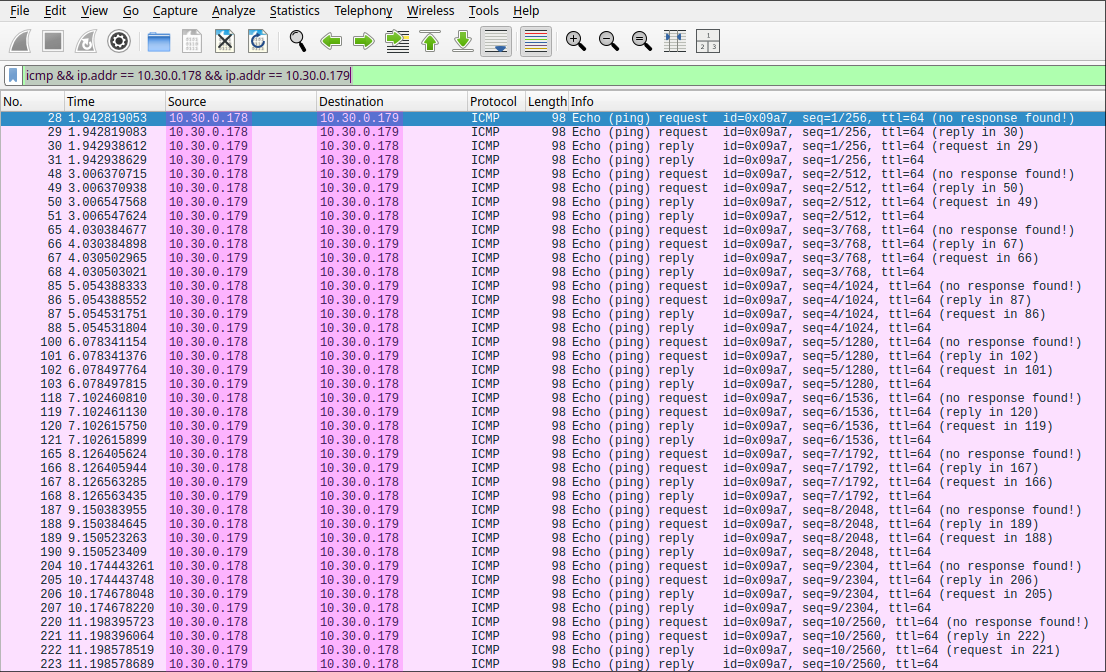
\includegraphics[scale=0.353]{images/whistBaa.png}
	\centering
	\caption{Observing a Ping Between Two Clients That Don't Involve the Attacker}
\end{figure} \abc \newpage
\subsection{Capturing Plain Text Passwords}
But let's not stop at having two targets ping each other—we can also make use of the web server VM, which is simply the default Nginx page protected with basic authentication. I already explained in detail how to set this up in Exercise 6, under the \say{Securing Nginx with Basic Authentication} section in my documentation for Exercise 6 \cite{exercise-6}.\abc
If we make a request to the HTTP server—using either a web browser, \texttt{curl}, or any other method—and pass the \texttt{Authorization} header, it will contain \texttt{Basic}, which is the scheme name, followed by a \texttt{Base64}-encoded \texttt{UTF-8} string of the username and password separated by a colon \texttt{:}, as described in RFC 7617 on pages 4 and 5~\cite{basic-auth-rfc}.\abc
The server then checks whether the provided credentials match an entry in the credentials file. If no match is found, as shown in Figure 11, an HTTP status code \texttt{401 Unauthorized} is returned. \cite{http-401}\abc
Since the attacker can view the target’s traffic, we can examine the provided credentials in the frame that sends the \texttt{GET} request to the server. This frame contains the \texttt{Authorization} header, which Wireshark conveniently and automatically decodes from \texttt{Base64} to \texttt{UTF-8}, revealing the credentials string in plain text, as shown in Figure 11 below.
\begin{figure}[!htbp]
	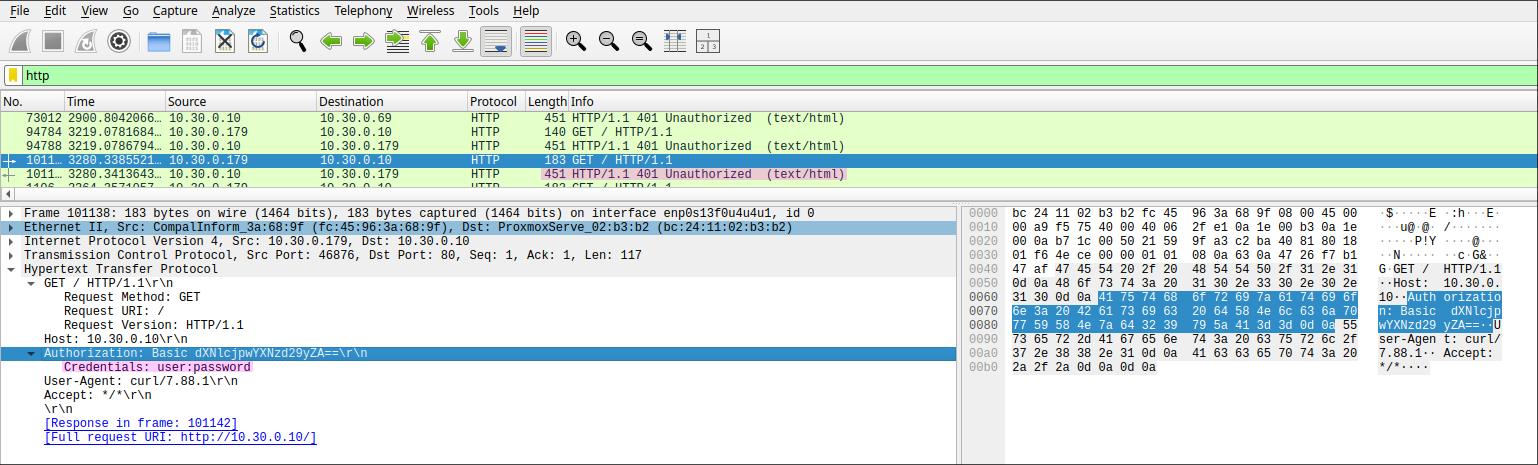
\includegraphics[scale=0.3]{images/hedah.png}
	\centering
	\caption{Viewing the plain text password from the authentication}
\end{figure} \abc 
Later, a successful authentication is made, where the server instead returns status code \texttt{200}, which indicates that the request has succeeded~\cite{http-200}.\abc
Again, we can see the credentials used in the request headers and now know that the credentials for this web server are \texttt{user3:password123}, as shown in Figure 12. In addition, we receive the entire HTML code returned in the response from the server, which we can also view in plain text—essentially allowing us to see the same content as the client, as shown in Figure 13.
\begin{figure}[!htbp]
	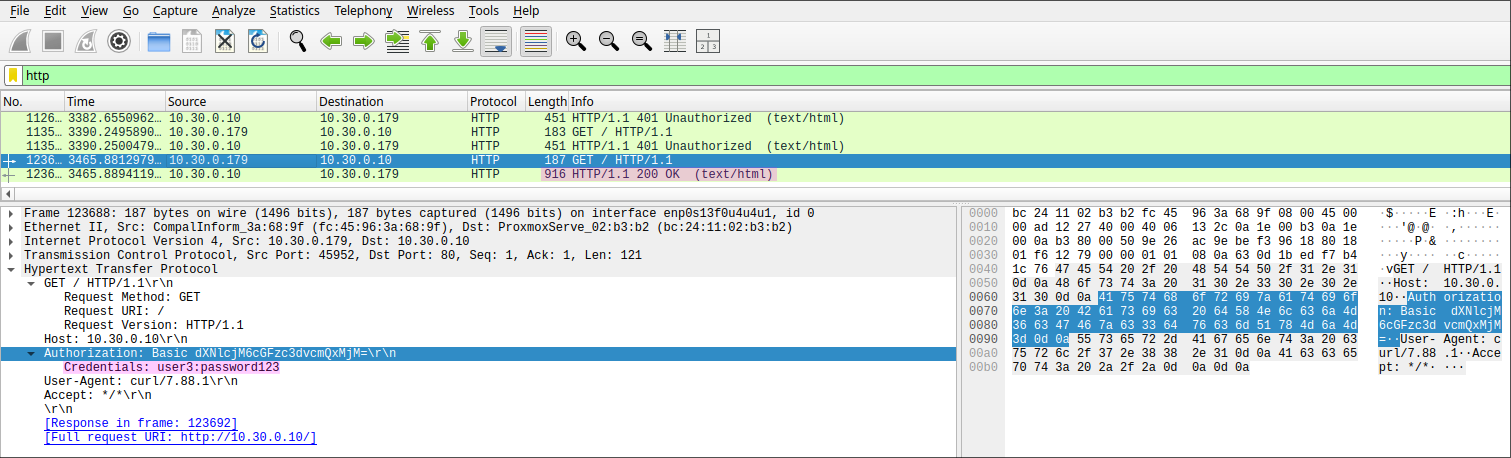
\includegraphics[scale=0.3]{images/headhgoog.png}
	\centering
	\caption{Viewing the correct plain text password from the authentication}
\end{figure} \abc \newpage
\begin{figure}[!htbp]
	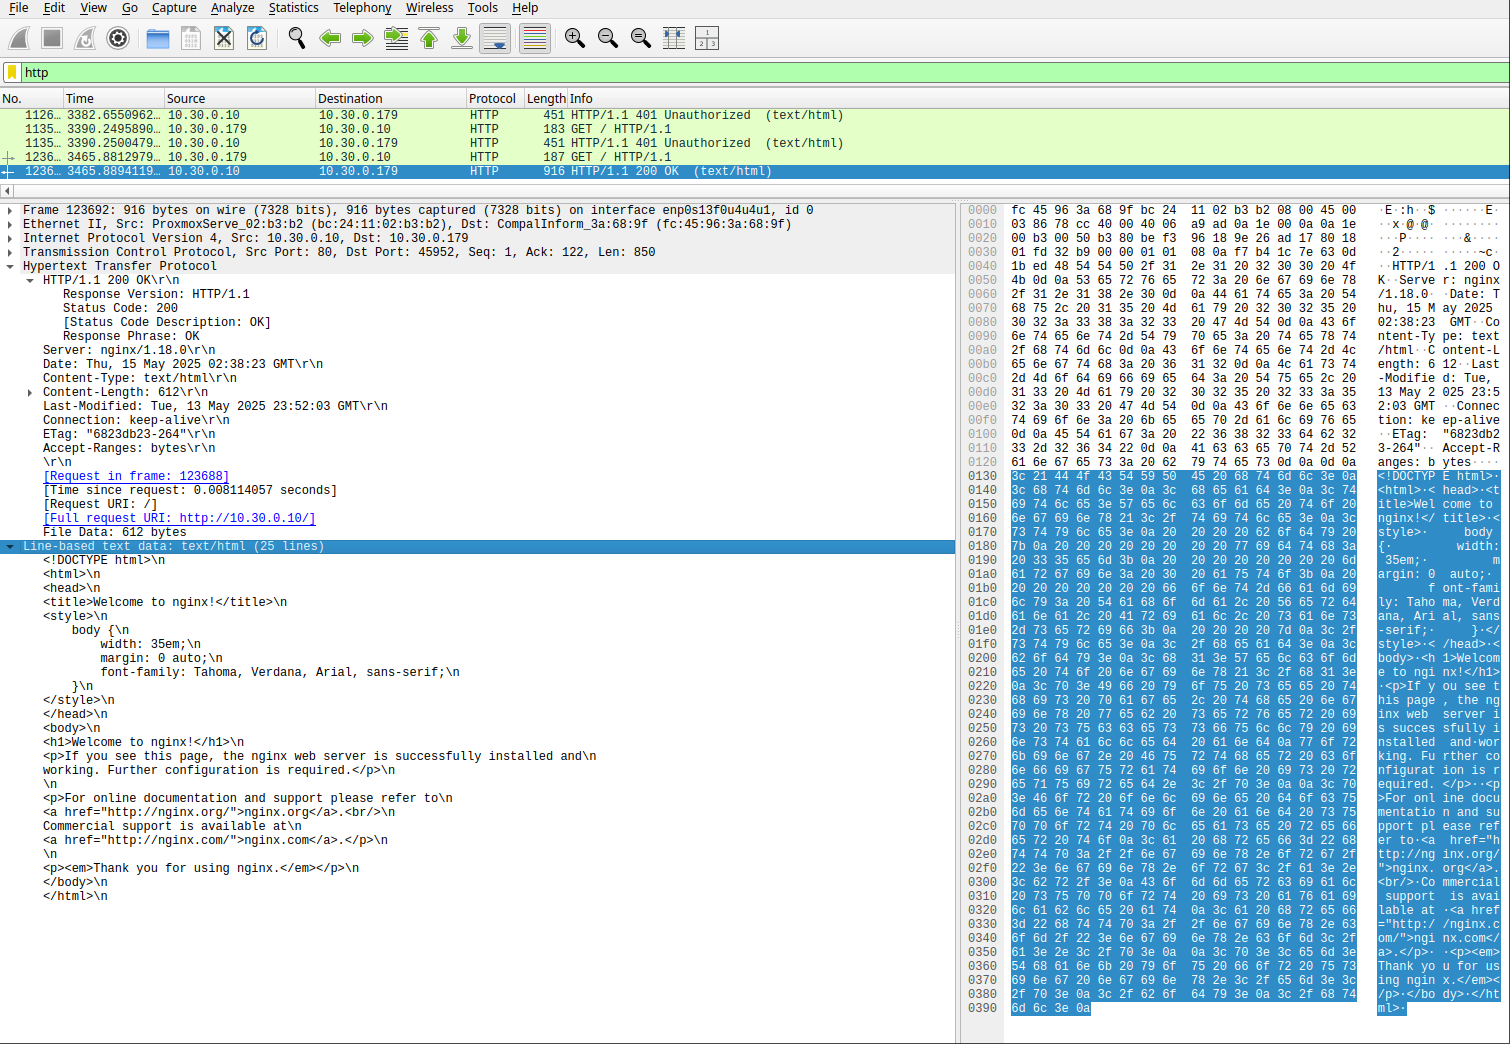
\includegraphics[scale=0.3]{images/eniterufcijsdigjsdg.png}
	\centering
	\caption{Viewing the returned \texttt{HTML}}
\end{figure} \abc
\subsection{Capturing a VoIP Call}
Lastly, \texttt{VoIP} traffic was captured and analyzed using Wireshark. For this, a different topology was used, as shown in \textcolor{blue}{\hyperref[fig:nwconf]{Figure \ref{fig:topo2}}}, since I do not own any \texttt{VoIP} phones. This part of the experiment was conducted in the school's networking lab, where we used a hub and the address range \texttt{10.0.0.0/24}. The attacker had the address \texttt{10.0.0.69}, while the two phones had \texttt{10.0.0.1} and \texttt{10.0.0.2}. Since a hub was used, no port mirroring had to be configured.\abc
Voice over IP is an unencrypted protocol that uses the \texttt{Real-time Transport Protocol (RTP)} to transmit application data, which Wireshark has built-in tools to follow and even convert back into audio~\cite{voip-wireshark, rtp}.\abc
Wireshark provides these tools under \texttt{Telephony} $\rightarrow$ \texttt{VoIP}, which automatically detects the relevant streams and identifies the speakers. In the window that opens (as shown in Figure 14 below), we have several options, such as viewing the Flow Sequence, which shows when the call was ringing and who was speaking when. However, we are more interested in the "Play Streams" button, which displays the waveform of the call (as shown in Figure 15), and allows us to export the audio as an MP3 file \cite{voip-wireshark}.\newpage
\begin{figure}[!htbp]
	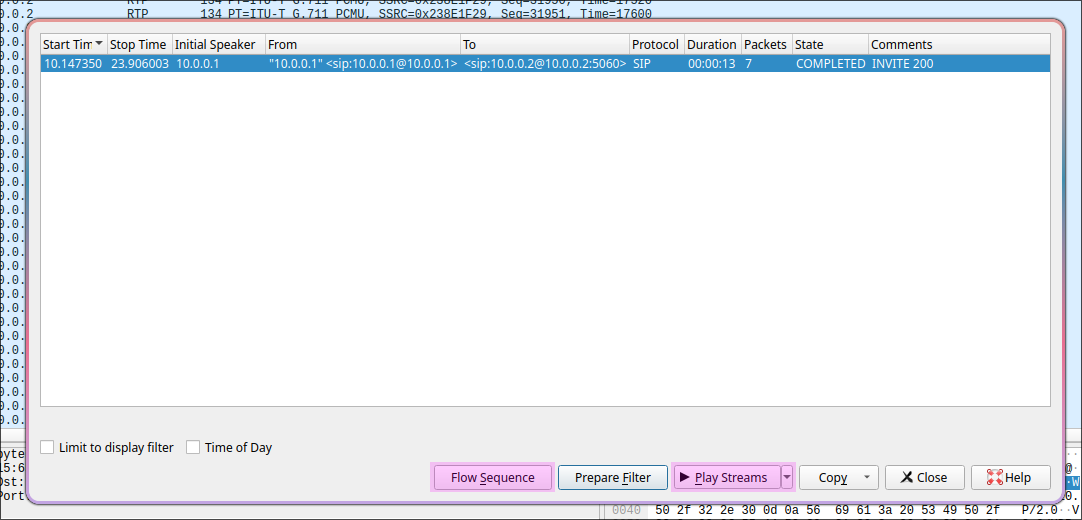
\includegraphics[scale=0.3]{images/phonedge.png}
	\centering
	\caption{Viewing the \texttt{VoIP} menu in Wireshark}
\end{figure} \abc
\begin{figure}[!htbp]
	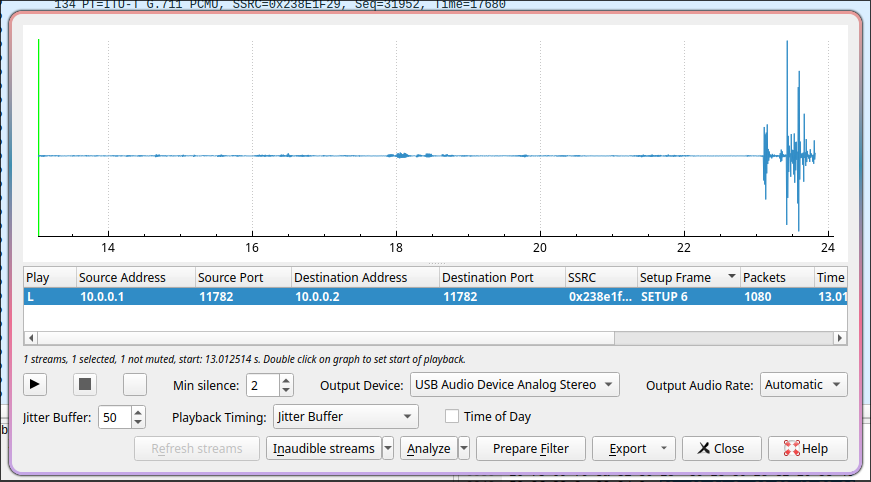
\includegraphics[scale=0.352]{images/waow.png}
	\centering
	\caption{Viewing the Waveform of the call}
\end{figure} \abc
However, the audio levels of the MP3 were initially unbalanced—the beginning was far too quiet—so I boosted the volume using Audacity, as shown in Figure 16, to normalize the audio levels. I then used the Adobe Podcast AI Audio Enhancer, as shown in Figure 17, to remove background noise and isolate the conversation. The result was a surprisingly clean and understandable audio file, even though the microphone of the other phone was quite far away when I was speaking. I'm actually quite surprised by the quality of the final result. \newpage
\begin{figure}[!htbp]
	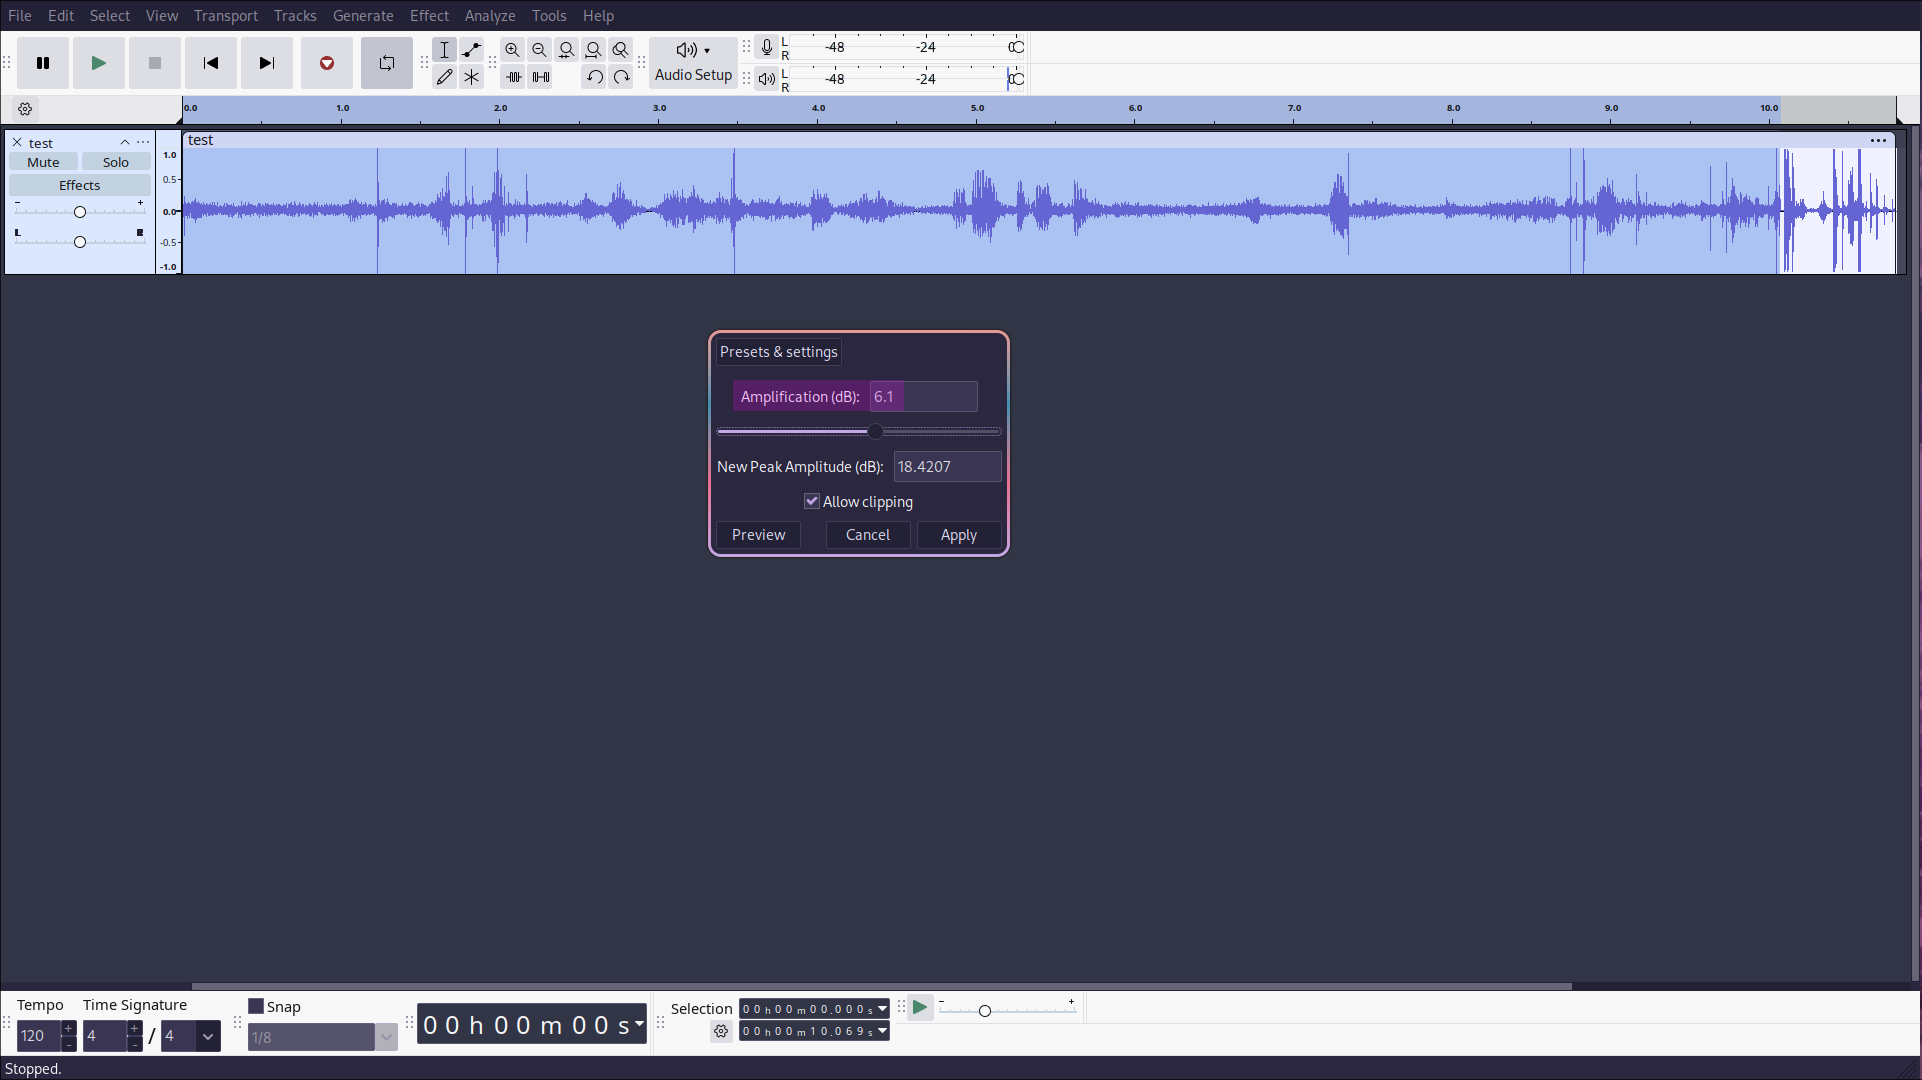
\includegraphics[scale=0.2]{images/fixing levels.png}
	\centering
	\caption{Fixing the Audio Levels in Audacity}
\end{figure} \abc
\begin{figure}[!htbp]
	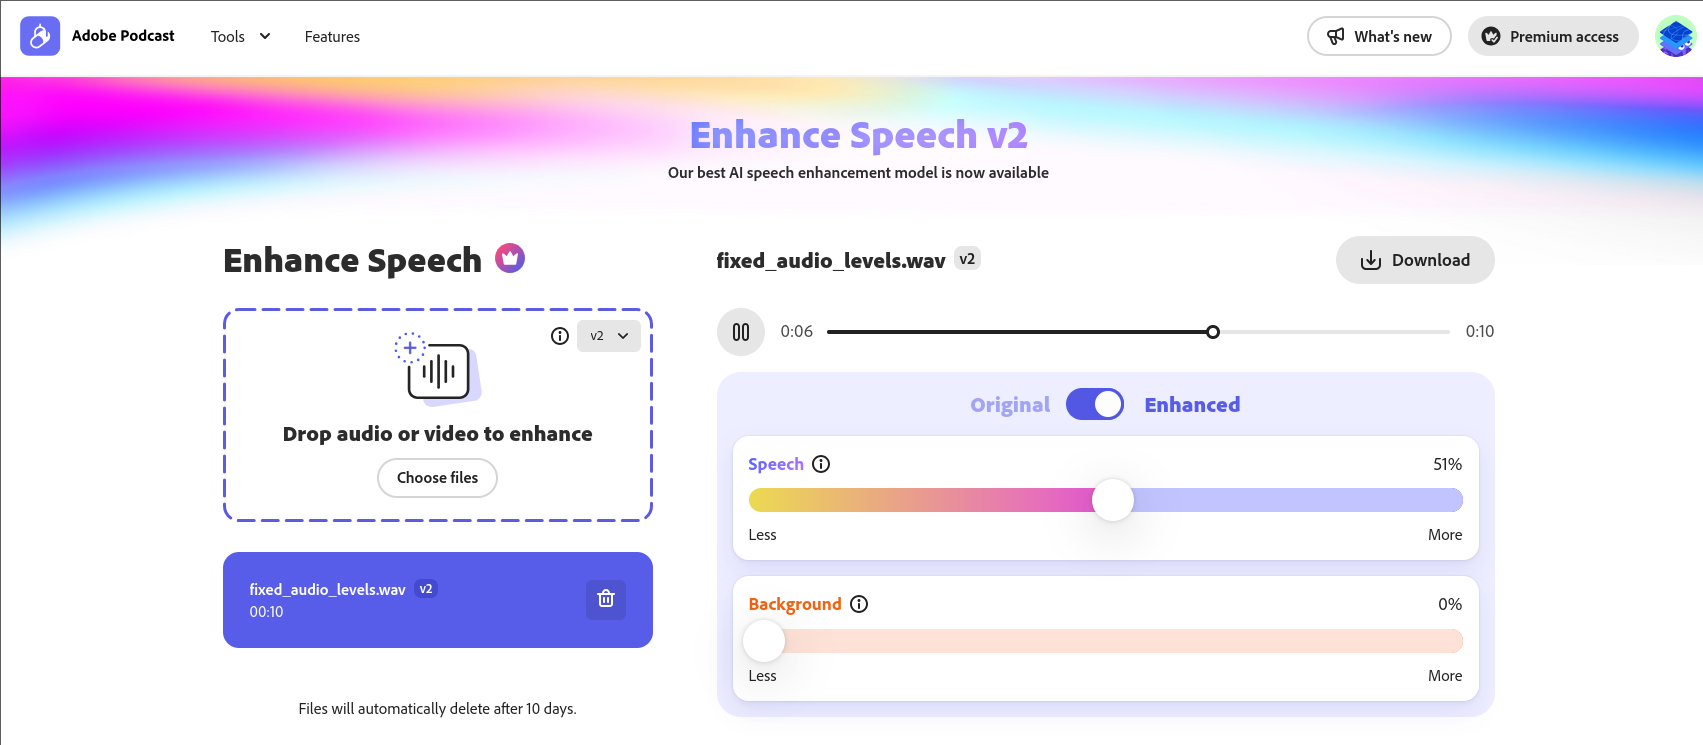
\includegraphics[scale=0.23]{images/adobe podcast.png}
	\centering
	\caption{Removing Background Noise Using Adobe's Podcast Tool}
\end{figure} \abc



\newpage
\section{References}
\bibliography{IEEEabrv,quellen}
\newpage
\section{List of figures}

\listoffigures

\end{document}
